\documentclass[11pt]{article}
\usepackage[margin=2.2cm]{geometry}
\usepackage{amsmath,amssymb,amsthm}
\usepackage{booktabs,array,longtable,multirow}
\usepackage{graphicx}
\usepackage{algorithm}
\usepackage{algpseudocode}
\usepackage{float}
\algtext*{EndWhile}\algtext*{EndFor}\algtext*{EndIf}
\usepackage[hidelinks]{hyperref}
\usepackage{enumitem}

% macros of the official template
\newcommand{\fillcell}{\rule{0pt}{2.2em}}
\newcommand{\fillrow}{\rule{0pt}{1.7em}}
\newcolumntype{C}[1]{>{\centering\arraybackslash}p{#1}}

\newtheorem{lemma}{Lemma}
\theoremstyle{remark}
\newtheorem*{remark}{Remark}
\newcommand{\fl}[1]{\left\lfloor #1\right\rfloor}
\newcommand{\cl}[1]{\left\lceil #1\right\rceil}
\newcommand{\E}{\mathrm{E}}
\newcommand{\ta}{\texttt{a}}
\newcommand{\tb}{\texttt{b}}
\newcommand{\tc}{\texttt{c}}
\setlength{\parskip}{0.35em}
\setlength{\emergencystretch}{2em}

\title{CMPE 300 Analysis of Algorithms\\[0.3em] \large Project 1 Report}
\author{Mert Seyhan (2023400213) \and Enes Ersoy (2023400039)}
\date{November 2026}

\begin{document}
\maketitle

\begin{abstract}
We analyse the given ``Example Algorithm'' for our variant (key $4$: $p_a=p_b=2/5$, $p_c=1/5$, $d=2$).
For each of the four basic-operation sets we derive the exact best-, worst- and average-case counts in closed form,
prove that the stated inputs are optimal, and give the asymptotic classes. We then implement the algorithm in Python,
identify group (4) as the operation set that characterises the running time, measure the execution time for 15 input
sizes, verify all exact counts with counters, and compare theory with measurements.
\end{abstract}

\tableofcontents
\newpage

%=====================================================================
\section{Introduction}
The project asks for a complete analysis of one algorithm: twelve exact analyses ($B$, $W$, $A$ for four
basic-operation sets), an implementation, timing experiments, exact count verification and a comparison of theory and
practice. We follow the analysis framework of the course (Slide01, pp.~3--9): fix the input size, fix the basic
operation, count, convert the count to a closed form, and express it asymptotically. The best- and worst-case proofs
use the per-iteration argument used for insertion sort (Slide03, pp.~6--7), and the average-case analyses use
$A(n)=\E[\tau]=\sum_i \E[\tau_i]$ (Slide03, p.~9) together with a first-order recurrence (Slide04) for the variable $s$.

Throughout, the input size is $n$, the length of \texttt{arr}. All numerical results in this report come from the calculations and
experiment data produced by the scripts in our project directory: the tables and figures are generated directly from
the result files, and the few values quoted in the text were taken from those files.

%=====================================================================
\section{Variant and Parameters}
Our student numbers are $No_1 = 2023400213$ and $No_2 = 2023400039$, so
\[
key = (2023400213 + 2023400039) \bmod 8 = 4046800252 \bmod 8 = 4 .
\]
(Since $1000$ is divisible by $8$, only the last three digits matter: $252 = 31\cdot 8 + 4$.) Row 4 of the variant
table gives:

\begin{center}
\begin{tabular}{|C{2.2cm}|C{2.2cm}|C{2.2cm}|C{2.2cm}|C{2.2cm}|}
\hline
\textbf{key} & $\boldsymbol{p_a}$ & $\boldsymbol{p_b}$ & $\boldsymbol{p_c}$ & $\boldsymbol{d}$ \\ \hline
\fillcell 4 & $2/5$ & $2/5$ & $1/5$ & $2$ \\ \hline
\end{tabular}
\end{center}


Each element is \ta{} with probability $2/5$, \tb{} with probability $2/5$ and \tc{} with probability $1/5$,
independently of the other elements, and the loop on line 7 divides by $d=2$. We first derive the results for general
$p_a,p_b,p_c,d$ where that is no harder, and then substitute our values.

%=====================================================================
\section{The Algorithm}
\begin{algorithm}[H]
\caption{Example Algorithm (as given in the project description)}
\begin{algorithmic}[1]
\Require $arr[0:n-1]$, integer $d$
\State $res \gets 0$;\ \ $s \gets 0$
\For{$i \gets 0$ \textbf{to} $n-1$}
  \If{$arr[i] = \ta$} \Comment{(1)}
    \State $s \gets s+1$ \Comment{(3)}
    \State $k \gets n$
    \While{$k>0$}
      \State $k \gets \fl{k/d}$ \Comment{(4)}
    \EndWhile
  \ElsIf{$arr[i] = \tb$} \Comment{(1)}
    \For{$q \gets 0$ \textbf{to} $s$} \Comment{(2)}
      \State $res \gets res + q$ \Comment{(3)}
      \For{$r \gets 1$ \textbf{to} $n$}
        \State $res \gets res + r$ \Comment{(4)}
      \EndFor
    \EndFor
  \Else \Comment{$arr[i]=\tc$}
    \State $s \gets 0$ \Comment{(3)}
    \For{$t \gets i$ \textbf{to} $n-1$} \Comment{(2)}
      \State $res \gets res+t$ \Comment{(4)}
    \EndFor
  \EndIf
\EndFor
\State \Return $res$
\end{algorithmic}
\end{algorithm}
The line numbers 1--17 of this listing are the same as in the project description.

\subsection{The four basic-operation sets}
\begin{itemize}[nosep]
\item[(1)] the comparisons $arr[i]=\ta$ (line 3) and $arr[i]=\tb$ (line 8);
\item[(2)] the loop increments of the loops on line 9 ($q$) and line 15 ($t$);
\item[(3)] the assignments $s\gets s+1$ (line 4), $res\gets res+q$ (line 10), $s\gets 0$ (line 14);
\item[(4)] the assignments $k\gets\fl{k/d}$ (line 7), $res\gets res+r$ (line 12), $res\gets res+t$ (line 16).
\end{itemize}
Line 5, the test of line 6 and the loop on line 11 are not marked and are not counted in any group.

Two conventions are needed to count exactly:
\begin{itemize}[nosep]
\item A comparison is counted each time it is \emph{evaluated}. Line 3 is evaluated in every iteration; line 8 only when
line 3 is false, i.e.\ when $arr[i]\in\{\tb,\tc\}$.
\item A loop ``\textbf{for} $q\gets 0$ \textbf{to} $s$'' is executed as $q\gets 0$; \textbf{while} $q\le s$:
body; $q\gets q+1$. Hence the increment is executed once per iteration, $s+1$ times. In the same way the loop on
line 15 performs $n-i$ increments.
\end{itemize}

\subsection{Two lemmas}
\begin{lemma}[the \texttt{while} loop]\label{lem:log}
For $n\ge1$ and an integer $d\ge 2$, the loop on lines 6--7 starting from $k=n$ executes line 7 exactly
\[
\lambda(n) = \fl{\log_d n}+1
\]
times. For our variant $\lambda(n)=\fl{\log_2 n}+1$. Moreover $1\le \lambda(n)\le n$.
\end{lemma}
\begin{proof}
Using $\fl{\fl{x}/d}=\fl{x/d}$ for real $x\ge 0$ and integer $d$, after $j$ executions of line 7 we have
$k=\fl{n/d^{j}}$. The body is executed for the $(j+1)$-st time iff $\fl{n/d^{j}}>0$, i.e.\ iff $d^{j}\le n$, i.e.\ iff
$j\le \log_d n$. So the body runs for $j=0,1,\dots,\fl{\log_d n}$, which is $\fl{\log_d n}+1$ times (this is the same
halving argument as for binary search, Slide02 pp.~29--30). Since $n\ge1$ we get $\lambda\ge 1$, and
$d^{\,n-1}\ge 2^{n-1}\ge n$ gives $\fl{\log_d n}\le n-1$, so $\lambda\le n$.
\end{proof}
For example $\lambda(1)=1$, $\lambda(5)=3$, $\lambda(10)=4$, $\lambda(100)=7$, $\lambda(400)=9$.

\begin{lemma}[the variable $s$]\label{lem:s}
Let $s_i$ be the value of $s$ at the start of iteration $i$. Then $s_0=0$ and
\[
s_{i+1} = \begin{cases} s_i+1 & arr[i]=\ta\\ s_i & arr[i]=\tb\\ 0 & arr[i]=\tc.\end{cases}
\]
Consequently $s_i$ equals the number of \ta's among $arr[\ell..i-1]$, where $\ell$ is the position just after the last
\tc{} before $i$ ($\ell=0$ if there is none). In particular $s_i\le$ (number of \ta's before position $i$), and $s_i$
depends only on $arr[0..i-1]$.
\end{lemma}
\begin{proof}
Line 4 is the only place where $s$ grows and line 14 the only place where it is reset; the \tb-branch does not change
$s$. The statement follows by induction on $i$.
\end{proof}
The important point is that $s$ is \emph{not} reset at each outer iteration: a \tb{} sees all the \ta's since the most
recent \tc, even if there are \tb's in between.

\subsection{Cost of one outer iteration}
Let $\tau_{g}$ be the number of operations of group $g$ for a given input, and $\tau_{g,i}$ the part performed in
outer iteration $i$, so that $\tau_g=\sum_{i=0}^{n-1}\tau_{g,i}$ (the ``consecutive steps'' view of Slide03, p.~9).
From the pseudocode and the two lemmas:

\begin{center}
\renewcommand{\arraystretch}{1.25}
\begin{tabular}{c|cccc|c}
\toprule
$arr[i]$ & $\tau_{1,i}$ & $\tau_{2,i}$ & $\tau_{3,i}$ & $\tau_{4,i}$ & $s_{i+1}$\\ \midrule
\ta & $1$ & $0$ & $1$ & $\lambda$ & $s_i+1$\\
\tb & $2$ & $s_i+1$ & $s_i+1$ & $n(s_i+1)$ & $s_i$\\
\tc & $2$ & $n-i$ & $1$ & $n-i$ & $0$\\ \bottomrule
\end{tabular}
\end{center}
For \tb: the $q$-loop has $s_i+1$ iterations, each with one increment, one line-10 assignment and $n$ executions of
line 12. For \tc: the $t$-loop runs for $t=i,\dots,n-1$, i.e.\ $n-i$ times, each with one increment and one line-16
assignment. Writing $n_a,n_b,n_c$ for the numbers of \ta's, \tb's and \tc's ($n_a+n_b+n_c=n$), we get
\begin{align*}
\tau_1 &= n_a + 2(n_b+n_c) = 2n-n_a, &
\tau_2 &= \sum_{i:\,arr[i]=\tb}(s_i+1) + \sum_{i:\,arr[i]=\tc}(n-i),\\
\tau_3 &= n_a+n_c+\sum_{i:\,arr[i]=\tb}(s_i+1), &
\tau_4 &= \lambda n_a + n\!\!\sum_{i:\,arr[i]=\tb}(s_i+1) + \sum_{i:\,arr[i]=\tc}(n-i).
\end{align*}

\paragraph{A pair-counting identity.} Call a pair $(j,i)$ with $j<i$ an \emph{a--b pair} if $arr[j]=\ta$,
$arr[i]=\tb$ and there is no \tc{} between them. By Lemma~\ref{lem:s}, $s_i$ is the number of a--b pairs ending at a
\tb{} at position $i$, hence
\begin{equation}\label{eq:pairs}
\sum_{i:\,arr[i]=\tb}(s_i+1) = n_b + P,\qquad P=\#\{\text{a--b pairs}\}\le n_a n_b .
\end{equation}

\paragraph{A worked example.} For \texttt{abcabcba} ($n=8$, $\lambda=4$) the values of $s$ seen by the three \tb's are
$1,1,0$, and the table gives $\tau_1=13$, $\tau_2=2+6+2+3+1=14$, $\tau_3=10$,
$\tau_4=4+16+6+4+16+3+8+4=61$. Our program prints exactly these counts (Section~\ref{sec:impl}).

%=====================================================================
\section{Theoretical Analysis --- Group (1): Comparisons}
\textbf{Basic operation:} the comparisons on lines 3 and 8. From the table, $\tau_{1,i}=1$ if $arr[i]=\ta$ and $2$
otherwise, independently of $s$; so $\tau_1 = 2n-n_a$.

\subsection{$B_1(n)$}
Every iteration evaluates line 3, so $\tau_{1,i}\ge 1$ and $\tau_1\ge n$ for every input of size $n$.
\textbf{Best-case input:} $\ta^n$ (all \ta's). Then line 8 is never evaluated and $\tau_1=n$. Since no input can do
fewer than $n$, this input is a best case and
\[
B_1(n)=n\in\Theta(n)\quad(c_1=c_2=1).
\]
It is the only best case, because any \tb{} or \tc{} adds a second comparison.

\subsection{$W_1(n)$}
Each iteration evaluates at most the two comparisons, so $\tau_1\le 2n$ for every input.
\textbf{Worst-case input:} $\tb^n$ (any input without \ta{} works, e.g.\ $\tc^n$ too). Both comparisons run in every
iteration, so $\tau_1=2n$, and no input does more:
\[
W_1(n) = 2n\in\Theta(n).
\]

\subsection{$A_1(n)$}
Let $X_i\in\{\ta,\tb,\tc\}$ be the random character at position $i$. Then $\tau_{1,i}=1+[X_i\ne \ta]$ and
\[
A_1(n)=\E[\tau_1]=\sum_{i=0}^{n-1}\big(1\cdot p_a + 2(p_b+p_c)\big)=(2-p_a)n = \Big(2-\frac25\Big)n=\frac{8n}{5}\in\Theta(n).
\]
The variable $s$ plays no role in this group. (Check: $n=1$ gives $\frac25\cdot1+\frac35\cdot2=\frac85$.)

%=====================================================================
\section{Theoretical Analysis --- Group (2): Loop Increments}
\textbf{Basic operation:} the increments of the loops on lines 9 and 15.
$\tau_{2,i}=0$ for \ta, $s_i+1$ for \tb, $n-i$ for \tc.

\subsection{$B_2(n)$}
Counts are non-negative, so $\tau_2\ge 0$. \textbf{Best-case input:} $\ta^n$, which never enters the loops on lines 9
and 15, so $\tau_2=0$:
\[
B_2(n)=0\in O(1).
\]
(The count is identically zero, so it is constant; strictly speaking $0\notin\Theta(1)$ because $\Theta$ requires an
eventually positive function, Slide01 p.~26, so we write $O(1)$.) The input is the unique best case: a \tb{}
contributes $s_i+1\ge1$ and a \tc{} contributes $n-i\ge 1$.

\subsection{$W_2(n)$}
\textbf{Worst-case input:} $\tc^n$. The \tc{} at position $i$ gives $n-i$ increments, so
$\tau_2=\sum_{i=0}^{n-1}(n-i)=\sum_{j=1}^n j=\frac{n(n+1)}{2}$.

\textbf{Proof that no input does more.} By \eqref{eq:pairs},
$\tau_2 = \sum_{arr[i]=\tc}(n-i)+n_b+P$. Each a--b pair $(j,i)$ is determined by $j$ and a later position $i$, so an
\ta{} at position $j$ belongs to at most $n-1-j$ pairs, giving $P\le\sum_{arr[j]=\ta}(n-1-j)$. Therefore
\[
\tau_2\le \sum_{arr[i]=\tc}(n-i)+\sum_{arr[i]=\tb}1+\sum_{arr[j]=\ta}(n-1-j)
\le \sum_{i=0}^{n-1}(n-i)=\frac{n(n+1)}{2},
\]
because $1\le n-i$ and $n-1-j< n-j$ for every position. Hence
\[
W_2(n)=\frac{n(n+1)}{2}\in\Theta(n^2)\qquad\Big(\tfrac12 n^2\le W_2(n)\le n^2\text{ for }n\ge1\Big).
\]
The second inequality is strict as soon as the input contains an \ta, so no input using \ta's can reach the maximum.
This shows that, for this group, mixing \ta's and \tb's does not help: a \tc{} early in the array is worth more than
any \tb.

\subsection{$A_2(n)$}
\label{sec:Es}
\textbf{Random variables.} $X_0,\dots,X_{n-1}$ are the independent characters, and $S_i$ is the value of $s$ at the
start of iteration $i$. By Lemma~\ref{lem:s}, $S_i$ is a function of $X_0,\dots,X_{i-1}$ only, so \emph{$S_i$ and
$X_i$ are independent}. This is the key fact that lets us handle the state $s$.

\textbf{Expectation of $S_i$.} Let $e_i=\E[S_i]$. Conditioning on $X_i$ (as in the MaxMin analysis, Slide05) and using
the independence of $S_i$ and $X_i$:
\[
e_{i+1}=p_a(e_i+1)+p_b\,e_i+p_c\cdot 0=(1-p_c)\,e_i+p_a,\qquad e_0=0 .
\]
This is a first-order linear recurrence (Slide04, Type 1). With $\rho=1-p_c$ (we write $\rho$ to avoid confusion with the loop variable $q$), backward substitution gives
\[
e_i = p_a + \rho\,e_{i-1} = p_a(1+\rho) + \rho^2 e_{i-2}=\dots=p_a\sum_{j=0}^{i-1}\rho^{j}=\frac{p_a}{p_c}\left(1-\rho^{i}\right).
\]
For our variant $\rho=4/5$ and $p_a/p_c=2$, so
\[
e_i=\E[S_i] = 2\left(1-\left(\tfrac45\right)^{i}\right),\qquad 0\le e_i<2 .
\]
(Check: $e_1=2/5=p_a$, and $e_2 = \frac45\cdot\frac25+\frac25=\frac{18}{25}$.) The same result follows from
indicators: $S_i=\sum_{j<i}I_j$ where $I_j=1$ iff $X_j=\ta$ and none of $X_{j+1},\dots,X_{i-1}$ is \tc; then
$\E[I_j]=p_a \rho^{\,i-1-j}$ and summing gives the same geometric series. We will need the sum
\[
\sum_{i=0}^{n-1}e_i=\frac{p_a}{p_c}\Big(n-\sum_{i=0}^{n-1}\rho^{i}\Big)=\frac{p_a}{p_c}\Big(n-\frac{1-\rho^{n}}{p_c}\Big)
=2n-10+10\left(\tfrac45\right)^{n}.
\]

\textbf{Expected cost of an iteration.} By linearity and the independence of $S_i$ and $X_i$,
\[
\E[\tau_{2,i}] = p_a\cdot 0 + p_b\,\E[S_i+1\mid X_i=\tb] + p_c\,(n-i) = p_b(e_i+1)+p_c(n-i).
\]
\textbf{Sum.}
\begin{align*}
A_2(n)&=\sum_{i=0}^{n-1}\big(p_b(e_i+1)+p_c(n-i)\big)
= p_b\Big(n+\sum_{i=0}^{n-1}e_i\Big)+p_c\frac{n(n+1)}{2}\\
&=\frac25\Big(3n-10+10\big(\tfrac45\big)^n\Big)+\frac{n(n+1)}{10}
=\frac{n^2}{10}+\frac{13n}{10}-4+4\left(\frac45\right)^{n}.
\end{align*}
(Check: $n=1$ gives $0.1+1.3-4+3.2=0.6=p_b\cdot1+p_c\cdot1$.)

\textbf{Asymptotic class.} Since $0<4(4/5)^n<4$: for $n\ge1$, $A_2(n)\le \frac{n^2}{10}+\frac{13n}{10}\le \frac{14}{10}n^2$;
for $n\ge 4$, $\frac{13n}{10}\ge 4$ so $A_2(n)\ge \frac{n^2}{10}$. Hence $A_2(n)\in\Theta(n^2)$ with $c_1=\frac1{10}$,
$c_2=\frac{14}{10}$, $n_0=4$. The quadratic term comes only from the \tc-loop; the \tb-loop contributes only
$O(n)$ because $\E[S_i]<2$.

%=====================================================================
\section{Theoretical Analysis --- Group (3): Assignments on Lines 4, 10, 14}
$\tau_{3,i}=1$ for \ta, $s_i+1$ for \tb, $1$ for \tc. Using \eqref{eq:pairs}:
\[
\tau_3=n_a+n_c+n_b+P = n+P .
\]

\subsection{$B_3(n)$}
Every iteration performs at least one of these assignments (line 4, line 14, or line 10 at least once since the
$q$-loop runs $s_i+1\ge 1$ times), so $\tau_3\ge n$. \textbf{Best-case input:} $\ta^n$, giving $\tau_3=n$. Thus
\[
B_3(n)=n\in\Theta(n).
\]
(Every input with $P=0$, e.g.\ $\tc^n$ or $\tb^n$, is also a best case; we use $\ta^n$.)

\subsection{$W_3(n)$}
\textbf{Worst-case input:} $\ta^{\fl{n/2}}\tb^{\cl{n/2}}$. Every \tb{} sees $s=\fl{n/2}$, so
$P=\fl{n/2}\cl{n/2}$ and $\tau_3=n+\fl{n/2}\cl{n/2}$.

\textbf{Proof that no input does more.} For any input $\tau_3=n+P\le n+n_an_b$, with $n_a+n_b\le n$. For a fixed
$n_a=x$ the bound $x\,n_b$ is largest when $n_b=n-x$, and
$x(n-x)=\frac{n^2}{4}-\big(x-\frac n2\big)^2$ is largest at the integer closest to $n/2$, where it equals
$\fl{n/2}\cl{n/2}=\fl{n^2/4}$. Hence $\tau_3\le n+\fl{n^2/4}$ for every input, and the input above attains it:
\[
W_3(n)=n+\left\lfloor\frac{n^2}{4}\right\rfloor\in\Theta(n^2).
\]
Bounds: $\fl{n^2/4}\ge (n^2-1)/4$ gives $W_3(n)\ge n^2/4$, and $W_3(n)\le n^2/4+n\le\frac54 n^2$ ($n\ge1$).
Note that here a \tc{} is never useful, because it adds only one operation and destroys the accumulated $s$.

\subsection{$A_3(n)$}
With the random variables of Section~\ref{sec:Es},
$\E[\tau_{3,i}] = p_a\cdot 1+p_b(e_i+1)+p_c\cdot1$, so
\begin{align*}
A_3(n)&=(p_a+p_c)\,n+p_b\Big(n+\sum_{i=0}^{n-1}e_i\Big)
=\frac35 n+\frac25\Big(3n-10+10\big(\tfrac45\big)^n\Big)
=\frac{9n}{5}-4+4\left(\frac45\right)^{n}.
\end{align*}
(Check: $n=1$ gives $1.8-4+3.2=1$, and indeed every input of size 1 performs exactly one of these assignments.)

\textbf{Asymptotic class.} $4(4/5)^n-4\le 0$, so $A_3(n)\le\frac95n$; and $A_3(n)\ge\frac95n-4\ge n$ for $n\ge5$.
Hence $A_3(n)\in\Theta(n)$, although $W_3(n)\in\Theta(n^2)$. The worst case needs $s$ to grow to about $n/2$, but on a
random input $s$ is reset by a \tc{} with probability $1/5$ in each step, and $\E[S_i]<2$.

%=====================================================================
\section{Theoretical Analysis --- Group (4): Assignments on Lines 7, 12, 16}
$\tau_{4,i}=\lambda$ for \ta, $n(s_i+1)$ for \tb, $n-i$ for \tc, where $\lambda=\fl{\log_2 n}+1$.

\subsection{$B_4(n)$}
\textbf{Lower bound for every input.} We bound each iteration separately:
\begin{itemize}[nosep]
\item \ta: $\tau_{4,i}=\lambda$;\quad \tc: $\tau_{4,i}=n-i$;
\item \tb: $\tau_{4,i}=n(s_i+1)\ge n\ge\max(\lambda,\,n-i)$ by Lemma~\ref{lem:log}.
\end{itemize}
So in every case $\tau_{4,i}\ge\min(\lambda,n-i)$, whatever the value of $s_i$, and
\[
\tau_4\ \ge\ \sum_{i=0}^{n-1}\min(\lambda,n-i)=\sum_{j=1}^{n}\min(\lambda,j)=\sum_{j=1}^{\lambda}j+(n-\lambda)\lambda
=n\lambda-\frac{\lambda(\lambda-1)}{2},
\]
where we substituted $j=n-i$ and used $\lambda\le n$.

\textbf{Best-case input:} $\ta^{\,n-\lambda}\tc^{\,\lambda}$. Positions $0,\dots,n-\lambda-1$ hold \ta{} and cost
$\lambda$ each (here $n-i>\lambda$), and positions $n-\lambda,\dots,n-1$ hold \tc{} and cost $n-i\in\{\lambda,\dots,1\}$.
There is no \tb, so $s$ does not matter. Every iteration attains its lower bound, so
\[
B_4(n)=n\lambda-\frac{\lambda(\lambda-1)}{2},\qquad \lambda=\fl{\log_2 n}+1 .
\]
For example $B_4(1)=1$, $B_4(10)=34$, $B_4(100)=679$.
\textbf{Asymptotic class.} $B_4(n)\le n\lambda$, and since $\lambda\le n$, $\frac{\lambda(\lambda-1)}{2}\le\frac{n\lambda}{2}$, so
$B_4(n)\ge\frac{n\lambda}{2}$. With $\log_2 n<\lambda\le\log_2 n+1\le 2\log_2 n$ for $n\ge 2$:
$\frac12 n\log_2 n\le B_4(n)\le 2n\log_2 n$, i.e.\ $B_4(n)\in\Theta(n\log n)$.

Intuitively, an \ta{} costs only $\lambda\approx\log_2 n$ operations, a \tc{} near the end of the array is even cheaper,
and a \tb{} always costs at least $n$; so the best input avoids \tb{} and uses \tc{} at the positions with $n-i\le\lambda$ (at $n-i=\lambda$ an \ta{} would
cost the same, so that position could hold either letter).

\subsection{$W_4(n)$}
\textbf{Upper bound for every input.} Using \eqref{eq:pairs}, $P\le n_an_b$ and $n-i\le n$:
\[
\tau_4=\lambda n_a+n(n_b+P)+\sum_{arr[i]=\tc}(n-i)\ \le\ \lambda n_a+n\,n_b+n\,n_an_b+n\,n_c .
\]
Put $x=n_a$ and $n_c=n-x-n_b$. The right side becomes $\lambda x+n(n-x)+n\,x\,n_b$, which does not decrease with $n_b$,
so it is at most its value for $n_b=n-x$:
\[
\tau_4\le f(x)=\lambda x+n(n-x)(x+1).
\]
Now we maximise $f$ over the integers $0\le x\le n$. The difference is
\[
f(x+1)-f(x)=\lambda+n\big[(n-x-1)(x+2)-(n-x)(x+1)\big]=\lambda+n(n-2x-2).
\]
If $x\le\fl{n/2}-1$ then $n-2x-2\ge0$ and the difference is $\ge\lambda>0$. If $x\ge\fl{n/2}$ then $n-2x-2\le-1$ and
the difference is $\le\lambda-n\le0$ (Lemma~\ref{lem:log}). So $f$ increases up to $x=\fl{n/2}$ and does not increase
after it, and $\tau_4\le f(\fl{n/2})$ for every input.

\textbf{Worst-case input:} $\ta^{\fl{n/2}}\tb^{\cl{n/2}}$. The \ta's cost $\lambda\fl{n/2}$ and each of the $\cl{n/2}$
\tb's sees $s=\fl{n/2}$ and costs $n(\fl{n/2}+1)$, which is exactly $f(\fl{n/2})$. Using
$\fl{n/2}\cl{n/2}=\fl{n^2/4}$:
\[
W_4(n)=\lambda\fl{\frac n2}+n\cl{\frac n2}\Big(\fl{\frac n2}+1\Big)
=n\fl{\frac{n^2}{4}}+n\cl{\frac n2}+\fl{\frac n2}\big(\fl{\log_2 n}+1\big).
\]
For example $W_4(1)=1$, $W_4(10)=320$, $W_4(100)=255350$.
\textbf{Asymptotic class.} For $n\ge2$: $W_4(n)\ge n\frac{n^2-1}{4}\ge\frac{n^3}{8}$, and
$W_4(n)\le\frac{n^3}{4}+\frac{n(n+1)}{2}+\frac n2\cdot n\le 2n^3$. Hence $W_4(n)\in\Theta(n^3)$.

The worst case is not a constant string: $\ta^n$ costs only $n\lambda$ and $\tb^n$ only $n^2$. It is the balance
between creating a large $s$ (\ta's) and using it (\tb's) that gives the cubic count, and a \tc{} would only destroy the
accumulated $s$.

\subsection{$A_4(n)$}
With the random variables of Section~\ref{sec:Es} and the independence of $S_i$ and $X_i$,
\[
\E[\tau_{4,i}]=p_a\lambda+p_b\,n\,(e_i+1)+p_c(n-i),
\]
so
\begin{align*}
A_4(n)&=p_a n\lambda+p_b n\Big(n+\sum_{i=0}^{n-1}e_i\Big)+p_c\frac{n(n+1)}{2}\\
&=\frac25 n\lambda+\frac25 n\Big(3n-10+10\big(\tfrac45\big)^n\Big)+\frac{n(n+1)}{10}\\
&=\frac{13n^2}{10}-\frac{39n}{10}+\frac{2n}{5}\big(\fl{\log_2 n}+1\big)+4n\left(\frac45\right)^{n}.
\end{align*}
(Check: $n=1$ gives $1.3-3.9+0.4+3.2=1$; every input of size 1 does exactly one such assignment.)

\textbf{Asymptotic class.} Upper bound for $n\ge1$: using $\lambda\le n$ and $4n(4/5)^n\le 4n\le 4n^2$,
$A_4(n)\le(\frac{13}{10}+\frac25+4)n^2$. Lower bound: dropping the positive terms,
$A_4(n)\ge\frac{13n^2}{10}-\frac{39n}{10}\ge n^2$ for $n\ge13$. Hence $A_4(n)\in\Theta(n^2)$, while
$W_4(n)\in\Theta(n^3)$ (see Section~\ref{sec:avgworst} for the reason).

%=====================================================================
\newpage
\section{Summary of Theoretical Results (Table 1)}
\subsection*{Table 1: Theoretical Analysis Results}
For each basic-operation set we give the exact closed-form count (for our variant) and its asymptotic class.
Here $\lambda=\fl{\log_2 n}+1$.

\begin{longtable}{|C{2.3cm}|C{1.5cm}|p{7.2cm}|C{3.0cm}|}
\hline
\textbf{Basic operation} & \textbf{Case} & \centering\arraybackslash\textbf{Exact count (closed form)} & \textbf{Asymptotic} \\ \hline
\endhead
\hline
\endfoot
% --- Case 1 ---
\multirow{3}{*}{\parbox{2.3cm}{\centering (1)\\comparisons}} & $B_1(n)$ & \fillcell $\displaystyle n$ & $\Theta(n)$ \\ \cline{2-4}
 & $W_1(n)$ & \fillcell $\displaystyle 2n$ & $\Theta(n)$ \\ \cline{2-4}
 & $A_1(n)$ & \fillcell $\displaystyle \frac{8n}{5}$ & $\Theta(n)$ \\ \hline
% --- Case 2 ---
\multirow{3}{*}{\parbox{2.3cm}{\centering (2)\\loop increments}} & $B_2(n)$ & \fillcell $\displaystyle 0$ & $O(1)\ (\text{constant } 0)$ \\ \cline{2-4}
 & $W_2(n)$ & \fillcell $\displaystyle \frac{n(n+1)}{2}$ & $\Theta(n^2)$ \\ \cline{2-4}
 & $A_2(n)$ & \fillcell $\displaystyle \frac{n^2}{10}+\frac{13n}{10}-4+4\left(\frac{4}{5}\right)^{n}$ & $\Theta(n^2)$ \\ \hline
% --- Case 3 ---
\multirow{3}{*}{\parbox{2.3cm}{\centering (3)\\assignments}} & $B_3(n)$ & \fillcell $\displaystyle n$ & $\Theta(n)$ \\ \cline{2-4}
 & $W_3(n)$ & \fillcell $\displaystyle n+\left\lfloor \frac{n^2}{4}\right\rfloor$ & $\Theta(n^2)$ \\ \cline{2-4}
 & $A_3(n)$ & \fillcell $\displaystyle \frac{9n}{5}-4+4\left(\frac{4}{5}\right)^{n}$ & $\Theta(n)$ \\ \hline
% --- Case 4 ---
\multirow{3}{*}{\parbox{2.3cm}{\centering (4)\\assignments}} & $B_4(n)$ & \fillcell $\displaystyle n\lambda-\frac{\lambda(\lambda-1)}{2},\ \ \lambda=\lfloor \log_2 n\rfloor+1$ & $\Theta(n\log n)$ \\ \cline{2-4}
 & $W_4(n)$ & \fillcell $\displaystyle n\left\lfloor \frac{n^2}{4}\right\rfloor+n\left\lceil \frac{n}{2}\right\rceil+\left\lfloor \frac{n}{2}\right\rfloor\left(\lfloor \log_2 n\rfloor+1\right)$ & $\Theta(n^3)$ \\ \cline{2-4}
 & $A_4(n)$ & \fillcell $\displaystyle \frac{13n^2}{10}-\frac{39n}{10}+\frac{2n}{5}\left(\lfloor \log_2 n\rfloor+1\right)+4n\left(\frac{4}{5}\right)^{n}$ & $\Theta(n^2)$ \\ \hline
\end{longtable}


\subsection{Independent checks of the twelve formulas}
\label{sec:mathcheck}
The proofs above are the justification. In addition we checked every formula in ways that do not reuse the program's
counting code (the script \texttt{verify\_math.py}; its log is in the \texttt{results} folder):
\begin{enumerate}[nosep]
\item A separate interpreter of the pseudocode (every \textbf{for} expanded into its \textbf{while} form, counts kept
per line number) was run on all $3^n$ inputs for $n=1,\dots,10$. The minimum and maximum of each group equal
$B_g(n)$ and $W_g(n)$, and the stated inputs attain them.
\item The exact expectation $\sum_I\tau(I)p(I)$ (Slide01, p.~12), computed with exact fractions over all $3^n$ inputs,
equals $A_g(n)$ for $n=1,\dots,9$.
\item A dynamic program over the states $(i,s)$ computes the exact minimum and maximum over all $3^n$ inputs without
using the best/worst-case proofs (it uses only the per-iteration cost table of Section 3.3, which was itself checked
against the interpreter on 300 random inputs); it agrees with $B_g(n)$ and $W_g(n)$ for every $n\le120$. A second dynamic program over the
distribution of $s$ gives the exact expectation, equal to $A_g(n)$ for $n\le40$ and $n=50,60,80,100,150$.
\item \texttt{sympy} derives $A_1,\dots,A_4$ symbolically from the general expressions and confirms the simplified forms
for $p_a=p_b=2/5$, $p_c=1/5$, as well as the leading constants ($A_2/n^2\to\frac1{10}$, $A_4/n^2\to\frac{13}{10}$,
$W_4/n^3\to\frac14$, $B_4/(n\log_2 n)\to1$).
\end{enumerate}
All checks passed with no mismatch.

%=====================================================================
\section{Implementation and Choice of the Basic Operation}
\label{sec:impl}
\subsection{Program}
The program \texttt{2023400213.py} (Python 3, standard library only) contains:
\begin{itemize}[nosep]
\item \texttt{algorithm(arr, d)}: a line-by-line translation of the pseudocode with no counters, used for timing. The
state $s$ is kept across iterations, $\fl{k/d}$ is Python's integer division \texttt{k // d}, and all loops have the
inclusive bounds of the pseudocode (\texttt{range(0, s+1)}, \texttt{range(1, n+1)}, \texttt{range(i, n)}).
\item \texttt{algorithm\_counted(arr, d)}: the same algorithm with four counters, one per group; it is used only in
count mode and for the count verification, never while timing.
\item input generators for the best and worst case of group (4) and random inputs with the variant distribution, and
the command-line interface described in the ReadMe.
\end{itemize}
In count mode, \texttt{python3 2023400213.py 2023400213 2023400039 --count abcabcba} prints
\begin{verbatim}
Variant: 4 (p_a=2/5, p_b=2/5, p_c=1/5, d=2)
Count(1): 13 Count(2): 14 Count(3): 10 Count(4): 61
\end{verbatim}
which agrees with the hand computation in Section~3. An automated test suite (72 tests) compares the program with the
independent interpreter on all inputs up to length 8 (for $d=2$ and $d=3$), checks the formulas and the
output format, and runs both program modes as a subprocess.

\subsection{The ``correct'' basic operation}
\label{sec:basicop}
A realistic basic operation must give a count that is within constant factors of the running time for every input
(Slide01, pp.~5--6). We claim that group (4) has this property and the other three do not.

\textbf{Group (4).} The three statements of group (4) are exactly the bodies of the three innermost loops (lines 6--7,
11--12 and 15--16). Every other statement is either executed once per outer iteration (lines 3--5, 8, 14, loop set-up)
or once per iteration of the $q$-loop (lines 9--11), and one $q$-iteration always contains $n\ge1$ executions of line
12. Hence the total number $T(I)$ of executed statements satisfies $\tau_4(I)\le T(I)\le c\,(n+\tau_4(I))$ for a
constant $c$. Since every outer iteration contributes at least one group-(4) operation ($\lambda\ge1$, $n\ge1$,
$n-i\ge 1$), $\tau_4\ge n$, and therefore $T(I)\in\Theta(\tau_4(I))$ for every input.

\textbf{Groups (1)--(3).} Group (1) does not see the loops at all. Groups (2) and (3) count the $q$-loop but not the
$r$-loop inside it, and none of them counts the \texttt{while} loop. For example, on $\tb^n$ group (2) counts only $n$
increments, but $n^2$ assignments of line 12 are executed; on $\ta^n$ groups (2) and (3) count $0$ and $n$, but the
\texttt{while} loop runs $n\lambda$ times. Consequently their best and worst inputs are not the inputs that run
fastest or slowest. Table A1 (a supplementary table, numbered A1 to avoid confusion with the official Tables 1--4) shows this directly: the worst-case input of group (2), $\tc^n$, has
twice as many loop increments as $\ta^{n/2}\tb^{n/2}$ but runs about 240 times faster.

\begin{table}[h]
\centering
\parbox{0.9\linewidth}{\centering Table A1: Measured time of each group's own best/worst input at $n=400$ and its four counts (\texttt{results/extremes\_timing.csv}).}\par\smallskip
\small
\begin{tabular}{cllrrrrr}
\toprule
group & case & input & time (s) & $c_1$ & $c_2$ & $c_3$ & $c_4$ \\ \midrule
(1) & best & $a^{n}$ & 1.62e-04 & 400 & 0 & 400 & 3600 \\
(1) & worst & $b^{n}$ & 5.32e-03 & 800 & 400 & 400 & 160000 \\
(2) & best & $a^{n}$ & 1.62e-04 & 400 & 0 & 400 & 3600 \\
(2) & worst & $c^{n}$ & 2.78e-03 & 800 & 80200 & 400 & 80200 \\
(3) & best & $a^{n}$ & 1.63e-04 & 400 & 0 & 400 & 3600 \\
(3) & worst & $a^{n/2}b^{n/2}$ & 6.74e-01 & 600 & 40200 & 40400 & 16081800 \\
(4) & best & $a^{n-\lambda}c^{\lambda}$ & 1.61e-04 & 409 & 45 & 400 & 3564 \\
(4) & worst & $a^{n/2}b^{n/2}$ & 6.74e-01 & 600 & 40200 & 40400 & 16081800 \\
\bottomrule
\end{tabular}

\end{table}

\textbf{Measurements.} For all 132 timed inputs with $n\ge40$ (best, worst and the 10 random inputs per size, 11 sizes) we
divided the measured time by each of the four counts (\texttt{results/summary.txt}). For group (4) the time per
counted operation stays between 31 and 86\,ns (ratio max/min $=2.8$), while for groups (1), (2), (3) the ratio
max/min is 3113, 90 and 40. So the theory and the measurements agree: group (4) is the basic operation that
characterises the algorithm, and Table 2 uses the best-case input $\ta^{n-\lambda}\tc^{\lambda}$ and the worst-case
input $\ta^{\fl{n/2}}\tb^{\cl{n/2}}$ of group (4). (The best inputs of groups (1)--(3), $\ta^n$, are almost the same
as that of group (4) and indeed run equally fast; the worst input of group (3) coincides with that of group (4).)

%=====================================================================
\section{Real Execution (Table 2)}
\subsection{Method}
\begin{itemize}[nosep]
\item \textbf{Machine:} MacBook Air (Apple M1, 8 cores, 16 GB RAM), macOS 15.5; \textbf{language:} Python 3.14.3
(CPython). The measurements were taken on a normal desktop session (a web browser and an editor were running; load
average about 3), so some noise from other processes is expected.
\item \textbf{Timer:} \texttt{time.perf\_counter()} (monotonic, resolution $\approx 42$\,ns). Only the call of
\texttt{algorithm} is inside the timed region; input generation, counting and printing are outside it. The garbage
collector is disabled while timing, as in the \texttt{timeit} module.
\item \textbf{Repetition:} small inputs run in a few microseconds, close to the timer resolution. Therefore one timing
round executes the same input repeatedly until at least 20\,ms have passed and takes the mean time per execution;
each reported value is the smallest of 3 such rounds (the usual \texttt{timeit} practice, since larger values come
from interference, not from the algorithm). For large inputs a round is a single execution. The algorithm itself is
not changed.
\item \textbf{Average case:} for each $n$, 10 random arrays with $P(\ta)=P(\tb)=0.4$, $P(\tc)=0.2$ were generated
and timed; the table shows their mean. All 10 individual times are printed by the program and stored in
\texttt{results/timing.csv}.
\end{itemize}
Our first run used a single round per measurement; several average-case runs at $n=80$--$100$ were 3--6 times slower
per operation than their neighbours, clearly because of other processes. That run is kept in
\texttt{results/archive\_first\_attempt/}; the values below come from the second run with the 3-round rule.

\newpage
\subsection*{Table 2: Real Execution Times}
Basic operation identified as the ``correct'' one: \underline{group (4): assignments on lines 7, 12, 16}\\[0.4em]
Programming language / machine: \underline{Python 3.14.3 / MacBook Air, Apple M1, 16 GB, macOS 15.5}

\begin{center}
\begin{tabular}{|C{1.6cm}|C{3.4cm}|C{3.4cm}|C{3.8cm}|}
\hline
$n$ & \textbf{Best (s)} & \textbf{Worst (s)} & \textbf{Average (s)} \\ \hline
1   & \fillcell 9.078476e-07 & 8.198168e-07 & 4.680986e-07 \\ \hline
5   & \fillcell 1.994714e-06 & 4.446847e-06 & 1.862892e-06 \\ \hline
10  & \fillcell 4.002042e-06 & 2.318149e-05 & 5.904401e-06 \\ \hline
20  & \fillcell 8.101407e-06 & 1.327762e-04 & 1.907875e-05 \\ \hline
40  & \fillcell 1.580157e-05 & 9.699643e-04 & 7.550492e-05 \\ \hline
50  & \fillcell 2.032707e-05 & 1.698472e-03 & 1.385848e-04 \\ \hline
60  & \fillcell 2.518433e-05 & 2.871401e-03 & 1.424515e-04 \\ \hline
80  & \fillcell 4.253494e-05 & 6.880820e-03 & 2.592867e-04 \\ \hline
100 & \fillcell 5.838873e-05 & 1.315827e-02 & 4.311189e-04 \\ \hline
150 & \fillcell 9.621294e-05 & 4.117925e-02 & 9.622582e-04 \\ \hline
200 & \fillcell 1.142673e-04 & 9.157683e-02 & 1.549437e-03 \\ \hline
250 & \fillcell 1.418501e-04 & 1.381152e-01 & 2.472684e-03 \\ \hline
300 & \fillcell 1.880787e-04 & 2.322020e-01 & 3.942793e-03 \\ \hline
350 & \fillcell 2.071147e-04 & 4.003792e-01 & 5.358849e-03 \\ \hline
400 & \fillcell 2.340397e-04 & 6.416885e-01 & 7.672464e-03 \\ \hline
\end{tabular}
\end{center}


%=====================================================================
\section{Exact Count Verification}
\subsection{Best and worst case (Table 3)}
For each group and each $n\in\{1,5,10,20,40,100\}$ we ran the counted version on the best and worst input of that
group (Sections 4--7) and compared the counter with the formula.

\newpage
\subsection*{Table 3: Exact Count Verification (Best and Worst Case)}
\begin{longtable}{|C{2.3cm}|C{1.2cm}|C{2.6cm}|C{2.6cm}|C{2.6cm}|C{2.6cm}|}
\hline
\textbf{Basic operation} & $\boldsymbol{n}$ & \textbf{Counted best} & \textbf{Formula $B(n)$} & \textbf{Counted worst} & \textbf{Formula $W(n)$} \\ \hline
\endhead
\hline
\endfoot
\multirow{6}{*}{\parbox{2.3cm}{\centering (1)\\comparisons}} & 1 & \fillrow 1 & 1 & 2 & 2 \\ \cline{2-6}
 & 5 & \fillrow 5 & 5 & 10 & 10 \\ \cline{2-6}
 & 10 & \fillrow 10 & 10 & 20 & 20 \\ \cline{2-6}
 & 20 & \fillrow 20 & 20 & 40 & 40 \\ \cline{2-6}
 & 40 & \fillrow 40 & 40 & 80 & 80 \\ \cline{2-6}
 & 100 & \fillrow 100 & 100 & 200 & 200 \\ \hline
\multirow{6}{*}{\parbox{2.3cm}{\centering (2)\\loop increments}} & 1 & \fillrow 0 & 0 & 1 & 1 \\ \cline{2-6}
 & 5 & \fillrow 0 & 0 & 15 & 15 \\ \cline{2-6}
 & 10 & \fillrow 0 & 0 & 55 & 55 \\ \cline{2-6}
 & 20 & \fillrow 0 & 0 & 210 & 210 \\ \cline{2-6}
 & 40 & \fillrow 0 & 0 & 820 & 820 \\ \cline{2-6}
 & 100 & \fillrow 0 & 0 & 5050 & 5050 \\ \hline
\multirow{6}{*}{\parbox{2.3cm}{\centering (3)\\assignments}} & 1 & \fillrow 1 & 1 & 1 & 1 \\ \cline{2-6}
 & 5 & \fillrow 5 & 5 & 11 & 11 \\ \cline{2-6}
 & 10 & \fillrow 10 & 10 & 35 & 35 \\ \cline{2-6}
 & 20 & \fillrow 20 & 20 & 120 & 120 \\ \cline{2-6}
 & 40 & \fillrow 40 & 40 & 440 & 440 \\ \cline{2-6}
 & 100 & \fillrow 100 & 100 & 2600 & 2600 \\ \hline
\multirow{6}{*}{\parbox{2.3cm}{\centering (4)\\assignments}} & 1 & \fillrow 1 & 1 & 1 & 1 \\ \cline{2-6}
 & 5 & \fillrow 12 & 12 & 51 & 51 \\ \cline{2-6}
 & 10 & \fillrow 34 & 34 & 320 & 320 \\ \cline{2-6}
 & 20 & \fillrow 90 & 90 & 2250 & 2250 \\ \cline{2-6}
 & 40 & \fillrow 225 & 225 & 16920 & 16920 \\ \cline{2-6}
 & 100 & \fillrow 679 & 679 & 255350 & 255350 \\ \hline
\end{longtable}


All 48 counted values are equal to the formula values. This is expected, since the proofs show that the stated inputs
attain the formulas exactly.

\newpage
\subsection{Average case (Table 4)}
For each group and $n\in\{10,40,100\}$ we generated $N=1000$ random inputs with the variant distribution, counted the
operations, and compared the sample mean with $A(n)$ (the exact values of $A(n)$ are rational numbers; they are shown
rounded to four decimals).

\subsection*{Table 4: Exact Count Verification (Average Case)}
\noindent Number of random inputs used for each $n$ ($N\ge 1000$): \underline{\hspace{1cm}1000\hspace{1cm}}

\begin{center}
\begin{longtable}{|C{2.3cm}|C{1.2cm}|C{3.4cm}|C{3.0cm}|C{2.8cm}|}
\hline
\textbf{Basic operation} & $\boldsymbol{n}$ & \textbf{Mean of counted values} & \textbf{Formula $A(n)$} & \textbf{Difference} \\ \hline
\endhead
\hline
\endfoot
\multirow{3}{*}{\parbox{2.3cm}{\centering (1)\\comparisons}} & 10 & \fillrow 16.040 & 16.0000 & +0.040 \\ \cline{2-5}
 & 40 & \fillrow 64.072 & 64.0000 & +0.072 \\ \cline{2-5}
 & 100 & \fillrow 160.045 & 160.0000 & +0.045 \\ \hline
\multirow{3}{*}{\parbox{2.3cm}{\centering (2)\\loop increments}} & 10 & \fillrow 19.485 & 19.4295 & +0.056 \\ \cline{2-5}
 & 40 & \fillrow 208.354 & 208.0005 & +0.353 \\ \cline{2-5}
 & 100 & \fillrow 1135.566 & 1126.0000 & +9.566 \\ \hline
\multirow{3}{*}{\parbox{2.3cm}{\centering (3)\\assignments}} & 10 & \fillrow 14.398 & 14.4295 & -0.031 \\ \cline{2-5}
 & 40 & \fillrow 67.065 & 68.0005 & -0.936 \\ \cline{2-5}
 & 100 & \fillrow 176.102 & 176.0000 & +0.102 \\ \hline
\multirow{3}{*}{\parbox{2.3cm}{\centering (4)\\assignments}} & 10 & \fillrow 111.546 & 111.2950 & +0.251 \\ \cline{2-5}
 & 40 & \fillrow 1982.014 & 2020.0213 & -38.007 \\ \cline{2-5}
 & 100 & \fillrow 12900.934 & 12890.0000 & +10.934 \\ \hline
\end{longtable}
\end{center}


\noindent\begin{minipage}{\linewidth}
\setlength{\parskip}{0.35em}
\textbf{Comment on the differences.} $A(n)$ is the expected value of the count, while the table shows the mean of 1000
samples, which is itself random. The differences are small (at most about 2\%), have both signs, and do not grow
systematically. To judge them we compare each difference with the standard error $\hat\sigma/\sqrt N$ of the sample
mean:
\begin{center}\small
\begin{tabular}{cccccc}
\toprule
group & $n$ & difference & relative difference & std.\ error $\hat\sigma/\sqrt N$ & difference / std.\ error \\ \midrule
(1) & 10 & +0.040 & +0.25\% & 0.049 & +0.82 \\
(1) & 40 & +0.072 & +0.11\% & 0.096 & +0.75 \\
(1) & 100 & +0.045 & +0.03\% & 0.156 & +0.29 \\
(2) & 10 & +0.056 & +0.29\% & 0.194 & +0.29 \\
(2) & 40 & +0.353 & +0.17\% & 1.542 & +0.23 \\
(2) & 100 & +9.566 & +0.85\% & 6.770 & +1.41 \\
(3) & 10 & -0.031 & -0.22\% & 0.130 & -0.24 \\
(3) & 40 & -0.936 & -1.38\% & 0.523 & -1.79 \\
(3) & 100 & +0.102 & +0.06\% & 1.087 & +0.09 \\
(4) & 10 & +0.251 & +0.23\% & 1.375 & +0.18 \\
(4) & 40 & -38.007 & -1.88\% & 21.272 & -1.79 \\
(4) & 100 & +10.934 & +0.08\% & 109.669 & +0.10 \\
\bottomrule
\end{tabular}

\end{center}
\end{minipage}

All differences are below 2 standard errors, which is what random sampling produces with high probability, so the
measurements agree with the formulas. Group (1) has very small differences because its count $2n-n_a$ varies little.
Groups (2) and (4) at larger $n$ show the largest absolute differences, because their counts have a large variance: the
cost of a \tb{} grows with $s$, and the cost of a \tc{} depends strongly on its position, so a few inputs with a long run
of \ta's followed by \tb's (or with early \tc's) move the mean noticeably. Increasing $N$ would shrink the differences
like $1/\sqrt N$; they would not become exactly zero.

%=====================================================================
\section{Comparison of Theoretical Analysis and Real Behaviour}
\subsection{Graphs}
Figure~\ref{fig:theory} shows the twelve theoretical counts. Figure~\ref{fig:times} shows the measured times of
Table 2. Figure~\ref{fig:fit} compares the measured times with the group-(4) counts multiplied by a fitted cost per
operation, and Figure~\ref{fig:ratio} divides the measured time by each of the twelve theoretical counts. Because time
(seconds) and counts (operations) have different units, we never put them on two different axes of one plot: we either
scale the count by a fitted constant (seconds per operation) or plot their ratio.

\begin{figure}[htbp]
\centering
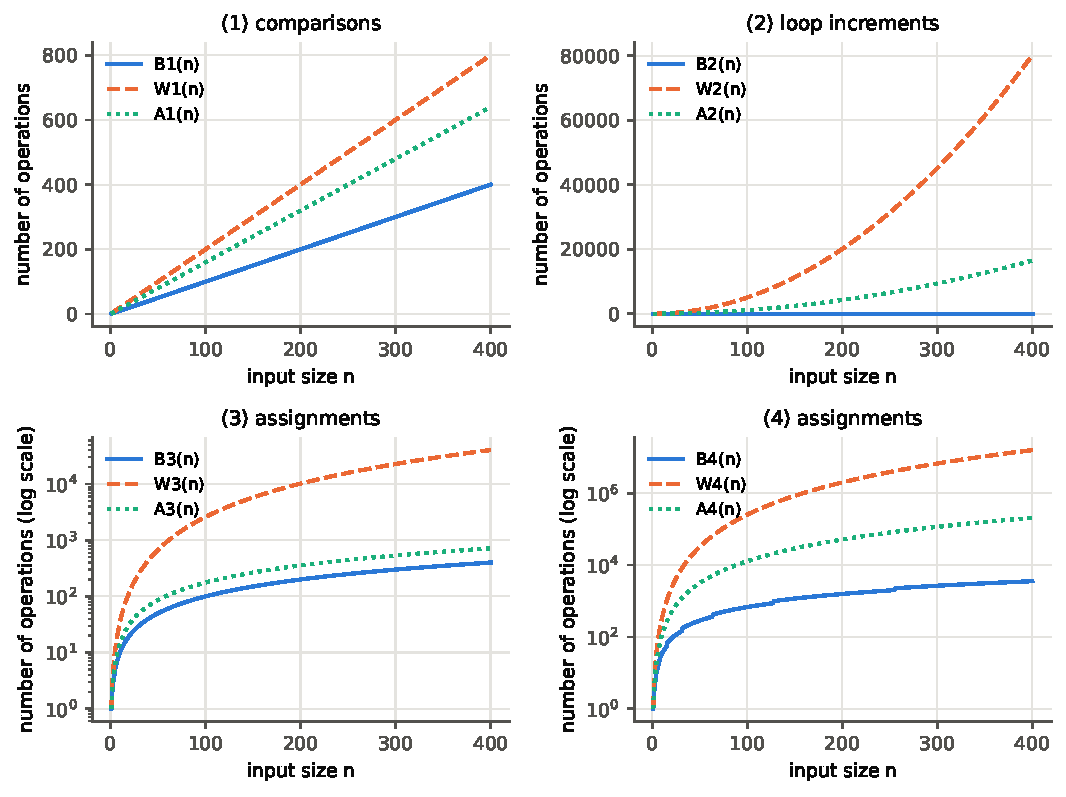
\includegraphics[width=0.92\textwidth]{../figures/theory_counts.pdf}
\caption{The twelve theoretical results $B_g(n)$, $W_g(n)$, $A_g(n)$ for $1\le n\le400$. Groups (3) and (4) use a
logarithmic $y$-axis; in group (2), $B_2(n)=0$ lies on the $x$-axis.}
\label{fig:theory}
\end{figure}

\begin{figure}[htbp]
\centering
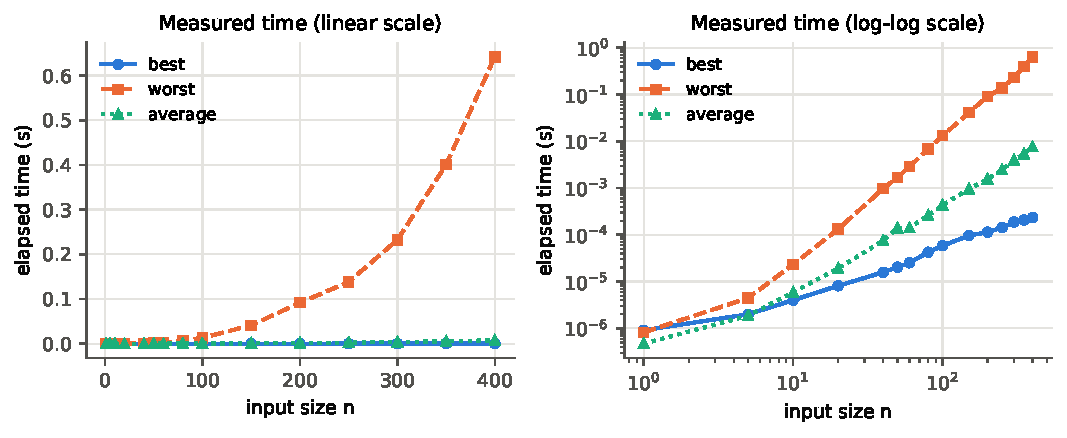
\includegraphics[width=0.92\textwidth]{../figures/measured_times.pdf}
\caption{Measured execution times (Table 2) on a linear and on a log-log scale.}
\label{fig:times}
\end{figure}

\begin{figure}[htbp]
\centering
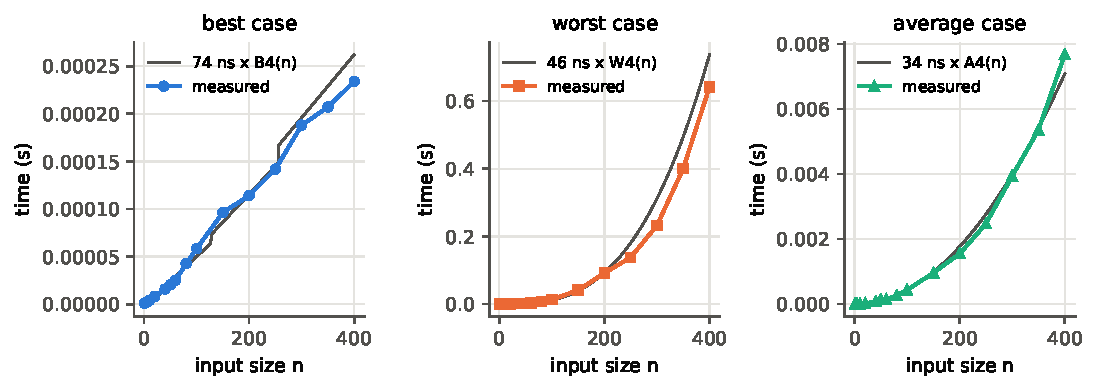
\includegraphics[width=0.95\textwidth]{../figures/group4_fit.pdf}
\caption{Measured times (markers) and $\alpha\cdot B_4(n)$, $\alpha\cdot W_4(n)$, $\alpha\cdot A_4(n)$ (lines), where
$\alpha$ is the mean time per operation over $n\ge40$ for that case.}
\label{fig:fit}
\end{figure}

\begin{figure}[htbp]
\centering
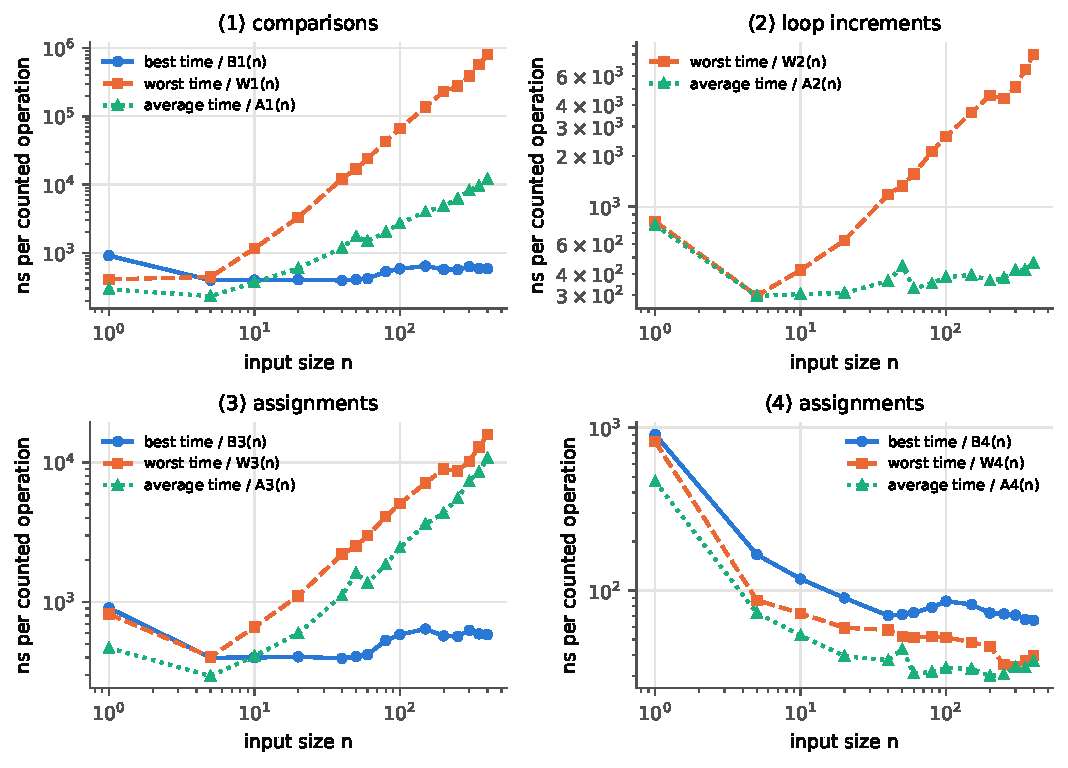
\includegraphics[width=0.92\textwidth]{../figures/time_per_operation.pdf}
\caption{Measured time divided by the theoretical count, for all twelve analyses (log-log). A curve that becomes flat
means the analysis predicts the growth of the running time. $B_2(n)=0$ cannot be used as a divisor and is omitted.}
\label{fig:ratio}
\end{figure}

\begin{figure}[htbp]
\centering
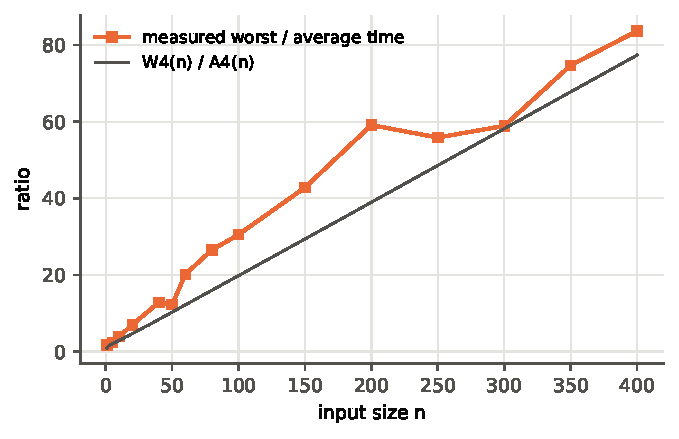
\includegraphics[width=0.55\textwidth]{../figures/worst_over_average.pdf}
\caption{Measured worst-case time divided by measured average-case time, together with $W_4(n)/A_4(n)$.}
\label{fig:wa}
\end{figure}

\subsection{Comments on each of the twelve analyses}
The best, worst and average times always refer to the inputs used in Table 2 (best/worst inputs of group (4), random
inputs for the average). Some comments quote empirical log-log slopes between $n=100$ and $n=400$. These are only rough
estimates from one recorded run and they vary from run to run: a later re-run of the program on the same machine
(\texttt{results/rerun\_2026-11-07\_normal\_mode\_output.txt}, not used in Table 2) gave slopes of $1.15$, $3.16$ and
$1.99$ for the best, worst and average case, against $1.00$, $2.80$ and $2.08$ in the recorded run. The asymptotic classes
themselves come from the proofs in Sections 4--7, not from these measurements.
\begin{description}[leftmargin=1.2em,style=nextline]
\item[$B_1(n)=n$, $\Theta(n)$.] The best-case time grows roughly linearly (empirical slope $1.00$ in the recorded
run, $1.15$ in the re-run), so $B_1$ is close to the growth of the best case for these sizes. This is a coincidence of this input: comparisons do not see
the \texttt{while} loop, but here that loop contributes only $\lambda\le 9$ operations per element.
\item[$W_1(n)=2n$, $\Theta(n)$.] Clearly wrong as a description of the slowest runs: the worst-case time grows almost
cubically while $W_1$ is linear, and time$/W_1$ in Figure~\ref{fig:ratio} grows by more than three orders of
magnitude. The worst input of group (1), $\tb^n$, is not even the slowest input (Table A1).
\item[$A_1(n)=8n/5$, $\Theta(n)$.] Also too small: the average time grows quadratically, so time$/A_1$ grows linearly.
\item[$B_2(n)=0$.] Says that the best input does no work, but the best-case run still takes time proportional to
$n\log n$ (or at least $n$). A zero count cannot describe running time.
\item[$W_2(n)=n(n+1)/2$, $\Theta(n^2)$.] Underestimates the worst-case time ($\Theta(n^3)$ measured), and its input
$\tc^n$ runs in $2.8$\,ms at $n=400$, versus $0.67$\,s for the real worst case.
\item[$A_2(n)$, $\Theta(n^2)$.] Has the same order, $\Theta(n^2)$, as the average time, and time$/A_2$ changes
much less than for groups (1) and (3) in Figure~\ref{fig:ratio} (it still rises by about $1.5\times$ between $n=10$ and
$400$). This agreement is only an accident: $A_2$ is dominated by the \tc-loop ($n^2/10$), whereas the average
time is dominated by the $r$-loop inside the \tb{} branch, which group (2) does not count.
\item[$B_3(n)=n$, $\Theta(n)$.] Same situation as $B_1$: right growth for the best-case time because the best input
contains no \tb.
\item[$W_3(n)=n+\fl{n^2/4}$, $\Theta(n^2)$.] Its worst input is the true slowest input, but the count is only
quadratic: each line-10 assignment hides $n$ assignments of line 12. Time$/W_3$ grows linearly.
\item[$A_3(n)=\frac95n-4+4(\frac45)^n$, $\Theta(n)$.] Predicts linear average behaviour, but the average time is
quadratic, for the same reason.
\item[$B_4(n)$, $\Theta(n\log n)$.] Figure~\ref{fig:fit} shows good agreement. The empirical slope ($1.00$ in the
recorded run, $1.15$ in the re-run) is somewhat below the count's slope between $n=100$ and $400$ ($1.20$). Part of this
is noise; a plausible additional reason is that each outer iteration also has a constant cost (the comparison,
$s\gets s+1$, $k\gets n$, loop overhead), which grows like $n$ and is comparable to $\lambda\le 9$ group-(4) operations
for these sizes, so the $\log n$ factor is hard to see for $n\le 400$.
\item[$W_4(n)$, $\Theta(n^3)$.] Matches the worst-case time well (Figure~\ref{fig:fit}); time$/W_4$ is almost flat
in Figure~\ref{fig:ratio}, at 34--58\,ns per operation for $n\ge 40$. The empirical slope between $n=100$ and $400$ is
$2.80$ in the recorded run and $3.16$ in the re-run, against $2.99$ for the count, so the difference is within the
run-to-run variation (see Section~\ref{sec:noise}).
\item[$A_4(n)$, $\Theta(n^2)$.] Matches the average time well; the empirical slope between $n=100$ and $400$ is
$2.08$ in the recorded run and $1.99$ in the re-run, against $2.01$ for $A_4$.
\end{description}
In short, only group (4) is consistent with the measurements in all three cases, which confirms the choice made in
Section~\ref{sec:basicop}.

\subsection{Average case versus worst case}
\label{sec:avgworst}
For the correct basic operation the average case is $\Theta(n^2)$ while the worst case is $\Theta(n^3)$, and the
measurements show the same gap: the worst/average time ratio is about 31, 59 and 84 at $n=100$, $200$ and $400$,
growing roughly linearly in $n$ like $W_4(n)/A_4(n)$ (Figure~\ref{fig:wa}). The reason is visible in the pseudocode.
A \tb{} costs $n(s+1)$ group-(4) operations, so the cost depends on $s$, the number of \ta's since the last \tc.
In the worst case there is no \tc{} at all, $s$ grows to $n/2$, and each of the $n/2$ \tb's costs about $n^2/2$
operations. In a random input, however, every position is a \tc{} with probability $1/5$, which resets $s$ to $0$
(line 14). Section~\ref{sec:Es} showed that $\E[S_i]=2(1-(4/5)^i)<2$: on average a \tb{} sees fewer than two \ta's,
so it costs fewer than $3n$ operations, and the $\approx 0.4n$ \tb's cost $\Theta(n^2)$ in total. The \tc's add
another $\Theta(n^2)$ through the loop on line 15, and the \ta's only $\Theta(n\log n)$. An input that keeps $s$
growing linearly needs long runs without \tc, and the probability of having no \tc{} at all is $(4/5)^n$, which
vanishes quickly. The ratio of the measured times is somewhat larger than $W_4/A_4$, because the cost per operation in
the worst case (about 46\,ns on average) is higher than in the average case (about 34\,ns), as seen in
Figure~\ref{fig:fit}.

\subsection{Small inputs and measurement noise}
\label{sec:noise}
For $n\le 10$ all three cases take 0.5--25\,$\mu$s, and the constant overhead of a Python function call and of the
loop set-up dominates; at $n=1$ the best-case input (\tc) even took slightly longer than the worst-case input (\tb),
although both perform one group-(4) operation. Asymptotic analysis ignores such constant costs
(Slide05, pp.~54--55), so it describes the measurements only from about $n\ge40$ on, where the time per group-(4)
operation becomes stable (Figure~\ref{fig:ratio}). The measurements also contain noise from other processes: for
example, the 10 average-case runs at $n=100$ differ by a factor of $2.85$ and the worst-case time per operation drops
from about 50\,ns ($n\le 200$) to about 35--40\,ns ($n\ge 250$). Part of the variation in the average case is real,
since the random inputs have different counts, but part of it comes from the machine. Neither effect changes the
growth rates, which agree with the analysis.

%=====================================================================
\section{Conclusion}
We derived exact closed forms for all twelve analyses and proved the optimality of every best- and worst-case input.
The comparisons (group 1) are $\Theta(n)$ in all cases; the loop increments (group 2) range from $0$ to $\Theta(n^2)$;
the assignments of group (3) are $\Theta(n)$, $\Theta(n^2)$ and $\Theta(n)$; and the innermost assignments of group (4)
are $\Theta(n\log n)$, $\Theta(n^3)$ and $\Theta(n^2)$. The state variable $s$ is what makes the worst case cubic, and
the resets of $s$ by \tc's (on average every fifth element) are what keep the average case quadratic. Group (4) is the
basic operation that characterises the running time: it counts the bodies of all innermost loops, and the measured time
per group-(4) operation is nearly constant over all inputs, while the other groups fail by large factors. All exact
counts were confirmed by counters, and the sample means of 1000 random inputs lie within two standard errors of the
average-case formulas.

\end{document}
